% !Rnw weave = knitr
\documentclass[12pt]{article}\usepackage[]{graphicx}\usepackage[]{color}
%% maxwidth is the original width if it is less than linewidth
%% otherwise use linewidth (to make sure the graphics do not exceed the margin)
\makeatletter
\def\maxwidth{ %
  \ifdim\Gin@nat@width>\linewidth
    \linewidth
  \else
    \Gin@nat@width
  \fi
}
\makeatother

\definecolor{fgcolor}{rgb}{0.345, 0.345, 0.345}
\newcommand{\hlnum}[1]{\textcolor[rgb]{0.686,0.059,0.569}{#1}}%
\newcommand{\hlstr}[1]{\textcolor[rgb]{0.192,0.494,0.8}{#1}}%
\newcommand{\hlcom}[1]{\textcolor[rgb]{0.678,0.584,0.686}{\textit{#1}}}%
\newcommand{\hlopt}[1]{\textcolor[rgb]{0,0,0}{#1}}%
\newcommand{\hlstd}[1]{\textcolor[rgb]{0.345,0.345,0.345}{#1}}%
\newcommand{\hlkwa}[1]{\textcolor[rgb]{0.161,0.373,0.58}{\textbf{#1}}}%
\newcommand{\hlkwb}[1]{\textcolor[rgb]{0.69,0.353,0.396}{#1}}%
\newcommand{\hlkwc}[1]{\textcolor[rgb]{0.333,0.667,0.333}{#1}}%
\newcommand{\hlkwd}[1]{\textcolor[rgb]{0.737,0.353,0.396}{\textbf{#1}}}%
\let\hlipl\hlkwb

\usepackage{framed}
\makeatletter
\newenvironment{kframe}{%
 \def\at@end@of@kframe{}%
 \ifinner\ifhmode%
  \def\at@end@of@kframe{\end{minipage}}%
  \begin{minipage}{\columnwidth}%
 \fi\fi%
 \def\FrameCommand##1{\hskip\@totalleftmargin \hskip-\fboxsep
 \colorbox{shadecolor}{##1}\hskip-\fboxsep
     % There is no \\@totalrightmargin, so:
     \hskip-\linewidth \hskip-\@totalleftmargin \hskip\columnwidth}%
 \MakeFramed {\advance\hsize-\width
   \@totalleftmargin\z@ \linewidth\hsize
   \@setminipage}}%
 {\par\unskip\endMakeFramed%
 \at@end@of@kframe}
\makeatother

\definecolor{shadecolor}{rgb}{.97, .97, .97}
\definecolor{messagecolor}{rgb}{0, 0, 0}
\definecolor{warningcolor}{rgb}{1, 0, 1}
\definecolor{errorcolor}{rgb}{1, 0, 0}
\newenvironment{knitrout}{}{} % an empty environment to be redefined in TeX

\usepackage{alltt}
\usepackage[backend=biber, sorting=nyt, maxcitenames=2, doi=false,url=false, style=apa]{biblatex} %add annotation=true and style=reading to print the annotations in the bibliography
\usepackage[american]{babel}
%\usepackage{newtxtext,newtxmath}
\usepackage{csquotes}
\bibliography{/Users/Owner/Documents/Tex/all,/Users/Owner/Documents/Thesis/thesis_ref}
\DeclareLanguageMapping{american}{american-apa}
\usepackage[compact]{titlesec}
\usepackage{csquotes}
\usepackage{amsmath}
%\usepackage[hyphens]{url}
\usepackage[margin=1in]{geometry}
\usepackage{mathtools}
\setlength{\parskip}{.6em}
\usepackage{setspace}
\usepackage{multicol}
\usepackage{longtable}
\usepackage{makecell}
\renewcommand\theadalign{bc}
\renewcommand\theadfont{\bfseries}
\renewcommand\theadgape{\Gape[4pt]}
\renewcommand\cellgape{\Gape[4pt]}
\renewcommand{\tablename}{Table}
%\usepackage{sectsty}
%\allsectionsfont{\singlespacing}
%\usepackage{indentfirst} %This indents the pfaragraph following a heading 
\setlength{\parindent}{0em}
\usepackage{breqn}
\usepackage{graphicx}
\usepackage{pdfpages}
\usepackage{subcaption}
\usepackage[figuresleft]{rotating}
\graphicspath{{C:/Users/Owner/documents/github/eysterthesis/manuscript/}} %make sure to include the slash after the colon at at the end 
%Make sure Bibliography --> is set as biblatex 
%Then run tools-->bibliography, then compile 
\usepackage{authblk}
\title{Invader success and changing climate: Comparisons in the native and introduced range of seven plant species}
\author[1]{Harold N. Eyster}
\author[2]{Elizabeth Wolkovich}
\affil[1]{Institute for Resources, Environment, and Sustainability, University of British Columbia}
\affil[2]{Department of Forest and Conservation Science, University of British Columbia}
\date{}                     %% if you don't need date to appear
\setcounter{Maxaffil}{0}
\renewcommand\Affilfont{\itshape\small}






\IfFileExists{upquote.sty}{\usepackage{upquote}}{}
\begin{document}
\maketitle
%	\fbox{\includegraphics[width=1 \textwidth,trim=0cm 0cm 0cm 0cm, clip=true]{comps_overview}}

\begin{spacing}{1} %1.9
	\begin{abstract}
		Invasive plants often have large impacts on ecosystems.  Yet we lack a clear understanding of how some species become successful invaders while others do not. Two competing techniques have been posited: 1) post-introduction rapid evolution or 2) broad environmental tolerance in the source population. These claims remain contested in part because distinguishing between them requires reciprocol common garden or growth chamber experiments, and these are relatively rare and typically only involve one or two species. Here, we use growth chambers to experimentally test the prevalence of post-introduction evolution in seven herbaceous plant species. Seeds were collected from multiple populations in their native (European) and invasive (North American) ranges. The seeds were subjected to one of two stratification treatments (to simulate different winter lengths) and then planted in growth chambers in one of four temperature treatments. Phenological traits were measured for each seed (germination rate, germination timing, and growth rate). Leveraging the flexibility of Bayesian multilevel models, we find only isolated effects of population origin. This suggests these exotic species need not evolve to become successful invaders. Instead, our results suggest that broad environmental tolderance is more important tham rapid evolution for granting invasion success. 
	\end{abstract}
\end{spacing}		
	\section{Introduction}
	Exotic plant invasions  can transform biodiversity \parencite{Bellard2016,Clavero2005,Walker1997}, and ecosystem function, services,and resilience \parencite{Daehler1999,Daehler1994,Ehrenfeld2003,Wilcove1998,Pejchar2009,Pimentel2005,Pysek2010,OTA1993,Mack2000,Levine2003}.  Yet we lack a clear understanding of what makes some species successful invaders and others not. This understanding is all the more important because invasions may only be increasing: globalization is making it easier for plants to disperse beyond their native ranges \parencite{Helmus2014,McKinney1999,Pysek2002,Vitousek1996,Wittenberg2001}. However, mere dispersal to a new environment is insufficient to entail invasiveness. Upon encountering a new environment, an invasive species must thrive, often by either filling vacant niches \parencite{Elton1958} or outperforming native plants in high-resource and variable environments \parencite{Davis2001,Daehler2003}. The availability of these invasible environments are likely to increase when ecosystems are altered \parencite{Tilman2001}. Anthropogenic greenhouse gas pollution and  habitat modification will likely disrupt communities and provide vacant niches and altered resource availability; such changes could provide major opportunities for invasive species to outperform native plants \parencite{Blois2013}. In particular, greenhouse gases are altering temperature, which is shifting temporal niche space and disrupting communities \parencite{Inouye2008,Harte2015}. This changing environment could select for species that can take advantage of the newly created temporal niches and resources through shifts in the timing of flowering and fruiting, etc. \parencite{Franks2007}. Two contrasting mechanisms have been posited to give some plants the capacity to exploit invasible environments: 1) post-introduction rapid evolution and 2) broad environmental tolerance in the source population. This paper tests the importance of these two mechanisms. 

	%To invade new The first factor for determining invasion potential is dispersal. To become invasive, a species first needs a dispersal mechanism to establish in a non-native habitat \parencite{Mark2001,Westphal2008}. Humans have played an important role in facilitating recent plant dispersals \parencite{McKinney1999,Pysek2002,Vitousek1996}, and with increased globalization the spread of species outside their respective native ranges will only increase \parencite{Helmus2014}. Once a species is introduced to a novel region, however, it must also be able to successfully disperse beyond the initial introduction location to be considered fully invasive. Thus species with greater dispersal ability may be more successful invaders.  Nonetheless, any intrinsic biological dispersal advantage can be wholly dominated by intentional introduction, e.g., for agricultural or ornamental purposes, or by accidental human-facilitated mechanisms, such as the transportation of invasive species within contaminated mulch or gravel \parencite{Wittenberg2001}. 	
	%Managing this onrush of invasive species requires understanding the mechanisms that give some plants the capacity to exploit invasible environments \parencite{Hulme2013}
	
	A large body of literature suggests that rapid adaptive evolution is a key driver of invasion success  \parencite{Sakai2001,Reznick2001, Lambrinos2004,Williamson1997,Thompson1998, Cox2004, Prentis2008,Colautti2015,Lee2002invasion, Fenollosa2019,Clements2011}.  Rapid evolution can enable nonindigenous species to adapt to vacant niches and take advantage of variable and high-resource environments, for example by evolving greater competitive ability  when released from natural enemies \parencite{Blossey1995,Bossdorf2005} or by evolving adaptive plasticity \parencite{Richards2006}. Many genetic characteristics have been identified to enable invasion, including additive genetic variation, epistasis, hybridization, genomic rearrangements, etc. \parencite[Reviewed in][]{Lee2002invasion}, while genetic drift and bottlenecks likely stifle invasion capacity \parencite{Bock2015}. 
	
	There are many clear examples of rapid evolution abetting plant invasions. For instance, genetic studies of two herbaceous goldenrods that invaded Europe from North America, \textit{Solidago altissima} and \textit{S. gigantea} (Asteraceae), showed post-introduction genetic changes in flowering time in response to temperature, due to selection on source-population genetic variation and development of new mutations \parencite{Weber1998}. Similarly, the invasive \textit{Centaurea solstitialis} (Asteraceae) in California evolved larger size from standing variation in the founding population \parencite{Barker2017}. Also in California, a similar study found that genetic adaptation was driving adaptive phenotypic variation in flowering time of high-altitude and desert populations of \textit{Capsella bursa-pastoris} (Brassicaceae) \parencite{Linde2001}. Invasion may even produce evolution sufficient to establish reproductive isolation and trigger speciation, in as few as 13 generations \parencite{Hendry2000}. If rapid evolution is so central to invader success, then managers should treat invasives not as static, homogeneous species, but as constantly adapting populations \parencite{Lee2002invasion}. 
	
	Yet, dispute the support for the importance of rapid evolution, a competing body of literature suggests that invaders need not evolve. Instead,  broad environemntal tolerance, plasticity and generalist adaptations to human-dominated environments (i.e., weediness) within the source population may give invaders sufficient advantages, obviating the necessity of rapid evolution \parencite{Richards2006,Schwartz1994,Bock2015,Rejmanek1996}. This is an longstanding theory. In 1965, Baker suggested that there were stable characteristics that made some species invasive: r-selected, high growth rates, broad environmental tolerance, etc. Species that are weedy in their native range are likely to be invasive in novel environments: a study of 274 plant species native to North and South America but naturalized in France showed that the best determinant of invasiveness was weediness in the home range \parencite{Maillet2000}. However, other studies found a lack of correlation between invasive traits and invasiveness \parencite{Perrins1992,Mack1996}, and studies that have found a relationship often failed to ensure that the invasive traits are present in native source populations. For example, a meta-analysis of 117 studies found that invasive plants were associated with performance-related traits, and concluded that it may be possible to predict future invaders by those traits \parencite{VanKleunen2010}. However, this reasoning ignores the possibility (as argued by the rapid evolution theory) that these performance-related traits only evolve post-introduction.  
	
	One reason why the importance of rapid evolution remains contested is because few experimental designs allow unambiguous discrimination between the two claims. Neither observational datasets (e.g., \parencite{Wolkovich2013} nor experimental common gardens \parencite{Conner2004,Vitasse2009} are sufficient to identify the importance of rapid evolution. And while genetic studies can identify the existence of rapid evolution, they do not demonstrate the dominance of this invasion technique. Instead, reciprocal common garden or  growth chamber experiments with native and invader populations are necessary to disentangle these competing theories. One such reciprocal common garden experiment of two invasive maple species (\textit{Acer}, Sapindaceae) demonstrated that rapid evolution was important for one species, but not the other \parencite{Lamarque2015}. Additional reciprocal common garden experiments have examined single species \parencite[e.g.,][]{Williams2008}. However, due to the limited number of species tested with these methods, the overall necessity of rapid evolution for invaders remains hidden.
	
	Seeking this more general appraisal of the importance of rapid evolution for invaders, this paper reports on a growth chamber experiment of the native and introduced ranges of seven highly invasive herbaceous plant species. We test the degree to which rapid evolution has occurred since the species colonized North America from Europe.  Our growth chamber experiment enabled us to test the degree to which phenologies in native and invasive populations differ in their response to climate.   Specifically, we measured how germination rate, time to germination, and growth rate of invasive (American) and native (European) conspecific populations responded to an array of temperature and stratification treatments.
	
	This study manipulates two key climate elements: temperature and stratification length. Temperature and stratification length act as important phenological cues for plants \parencite{Finch2006}. In temperate ecosystems, a cold stratification simulates winter. A minimum period of winter must often pass before seeds can germinate. This ensures that seeds will not germinate during a mid-winter warm period, but instead wait until a spring warm period when winter has fully passed. Thus, exposing dormant seeds to a variety of stratification lengths elucidates how they respond to different winter lengths. Once the necessary stratification length has been achieved, temperature can cue that it is the appropriate time for a seed or plant to break dormancy. Temperature also plays an important role in controlling plant growth rate \parencite{Egli1980,Guilioni2003}.
	
	Temperature and stratification length are appropriate variables for studying invasive vs. native plant phenology. These abiotic factors effectively trigger phenology, and can simulate diverse geographic environments. Additionally, temperature and stratification reflect different aspects of the seasonal environment: stratification length is associated with winter, while warmer temperatures are associated with the growing season. Including drivers such as stratification from the non-growing season is important, given that winter climate may change independently from summer climate, and that winter climate varies more spatially \parencite{Bonan2003}. Thus, a range of temperature and stratification treatments will simulate the driving features of the diverse environments in which invasive species thrive. 
	
	 If rapid evolution is of generalizable importance to invasive plants, we expect to find that seeds from the invading populations (North America) will respond very differently to temperature and stratification treatments than the indigenous populations (Europe) for all or nearly all species. Isolating the importance of rapid evolution in such a complex multispecies, multi-population design would be intractable with classic frequentest modeling  techniques. Fortunately, advances in Bayesian and multilevel modeling have provided methods that enable interpretation of our data \parencite{Carpenter2017}.  These experimental and statistical methods will provide a robust test of the claim that rapid evolution drives invader success.
	 
	\section{Methods}
	\subsection{Study species}
	%can probably cut: 
	There is no consensus on how to classify a species as invasive \parencite{Colautti2004}. The most common terms include `exotic,' `introduced,' `naturalized,' `nonindigenous,' `established,' `alien,' `noxious,' `weedy,' and `invasive.' These terms can be grouped into those that describe the provenance of the species (e.g., exotic, introduced, alien, non-indigenous), those that describe its ability to grow and compete in the new ecosystem (e.g., naturalized, established), and those that describe its impact on the receiving ecosystem (e.g., noxious, weedy, harmful). The International Union for the Conservation of Nature (IUCN, 2008) describes invasive species as: ``organisms introduced by man [sic] into places out of their natural range of distribution, where they become established and disperse, generating a negative impact." \nocite{IUCN2008is} However, this definition contains three subjective elements: what timepoint of a species' range is `natural,' whether humans are a natural part of nature, and what is defined as a negative impact \parencite{Munro2019}. To both acknowledge and allay some of these subjective elements, this paper will follow Richardson et al.'s \parencite{Richardson2000,Richardson2011} definition of invasive species. Invasive species are thus those that (1) are introduced across a previously unpenetrated barrier, (2) successfully reproduce in the place of introduction to create a stable local population, and finally (3) spread to produce fit offspring a substantial distance from the place of introduction.
	
	Guided by this definition, seeds were collected from eight herbaceous species that originated in Europe but have recently been introduced to the US, where they have spread and produced significant populations:\textit{ Alliaria petiolata, Capsella bursa-pastoris, Chelidonium majus, Dactylis glomerata,  Plantago lanceolata, P.  major, Rumex crispus, and Taraxacum officinale}. \textit{A. petiolata} exhibited very low germination rates, and so was removed from the analysis.  All of these species have proven prodigious invaders in the US, with many impacting crop production and transforming ecosystems \parencite[e.g.,][]{Froese2003,Wolfe2008}. The study species were selected for their occurrence in Europe and for their superior invasive capacity in their introduced range \parencite{Uva1997}, since the most unambiguous response may be obtained by examining the most extreme invasive species, and may also be most useful for informing management. 
%	\begin{center}
%		\begin{table}
%			\centering
%			\caption {Total number of seed-producing individuals and populations from which seeds were collected. Species are coded as the first three letters of the genus plus the first three letters of the species epithet.} \label{tab:seeds}  
%			\begin{tabular}{|c|c|c|c|}
%				\hline 
%				\makecell{\textbf{US} \\ \textbf{populations}} & \makecell{\textbf{US} \\  \textbf{individuals}} & \makecell{\textbf{European} \\ \textbf{populations}} & \makecell{\textbf{European} \\ \textbf{individuals}} \\
%				\hline
%				3&	21&	13&	63\\
%				\hline
%			\end{tabular}
%		\end{table}
%	\end{center}
	\subsubsection{Study species details}
	\textit{Capsella bursa-pastoris} (CAPBUR; Shepard's Purse) is an annual or biennial herbaceous plant in Brassicaceae. It grows 10 to 80 cm tall, typically blooming in late spring \parencite{Defelice2001}. It originated in Europe, and was introduced to the New World as a medicinal herb---it is now found across Canada, the US, and Mexico \parencite{Westrich1989}.
	
	\textit{Chelidonium majus} (CHEMAJ; Greater Celandine) is an herbaceous biennial member of Papaveraceae. It is native to Eurasia and North Africa and was introduced to the US by the 1670s as a medicinal. It is now found across the Eastern US and Canada and portions of the west \parencite{Holm1979}. 
	
	\textit{Dactylis glomerata} (DACGLO; Orchard Grass) is a cool-season, perennial grass (Poaceae). Plants grow up to 120 cm tall and have roots up to 60 cm long \parencite{Moser1996}. This plant originated in central and western Europe, and was intentionally introduced into the US in the 1750s \parencite{Bush2012} as a forage grass for pasture and hay \parencite{Ogle2011}.  
	
	\textit{Plantago lanceolata} (PLALAN; Narrow-leaved Plantain) is a perennial member of  Plantaginaceae. It has narrow, ribbed leaves and grows to 1m tall. It is native to Eurasia, and has successfully colonized the world's mid-latitudes \parencite{Holm1977}.
	
	\textit{Plantago major} (PLAMAJ; Broad-leaved Plantain) is a perennial member of Plantaginaceae. It has broad, smooth leaves, and grows to 15cm tall. Native to Europe, it was introduced into North America for its medicinal uses \parencite{Knobloch1996,Samuelsen2000}.
	
	\textit{Rumex crispus} (RUMCRI; Curly Dock) is a perennial herbaceous plant in Polygonaceae, and grows to 160 cm. It is native to Europe, Asia, and Africa, and was introduced for its medicinal uses into North America where it now found across much of the continent \parencite{USDA2010}. 
	
	\textit{Taraxacum officinale} (TAROFF; Dandelion) is a perennial herbaceous plant in the Asteraceae family, and grows to 60 cm. It is native to Eurasia, but is now found in all 50 US states, much of Canada, and Mexico \parencite{USDA1971}.
	
	\subsection{Seed collection}
	Seeds were collected from native populations in Europe and invasive populations in North America from June 15th to September 5th 2015. Mature seeds were collected from individual plants and placed into paper coin envelopes. The following data were recorded for each individual plant: species, date, name of site, notes on human disturbance at site, abundance of the species at the site, aspect, elevation, GPS coordinates, height of the individual, spread of the individual, photo of the site, photo of at least one individual/site, and soil type. The seeds were then stored at standard room temperature until early September 2015, at which time all of the seeds were cleaned and returned to envelopes. 
	\paragraph{European (native) seed collection} 
	Seeds were collected in Europe from early-June to mid-July 2015 from 63 individuals across 13 sites in 9 European countries: France, The Netherlands, Germany, Denmark, Norway, Austria, Slovenia, Liechtenstein, and Switzerland (see Figure \ref{fig:sites}). Seeds from European populations were collected from elevations ranging from sea level  to 1202 m (see Figure 2). Plant seeds were imported into the United States with a USDA small seedlot permit, which required that no more than 50 seeds be collected per envelope. Thus, typically 50 seeds/individual were collected. 
	
   \paragraph{North American (nonnative) seed collection} Seeds were collected in North America from June through early September from 21 individuals across three sites in Massachusetts, United States:  Harvard Forest (N 42.53096, W -72.19085), Arnold Arboretum at Harvard University, Boston (N 42.30196, W -71.12448), and Walden Pond, Concord (N 42.43927, W -71.3441) (see Figure \ref{fig:sites}). These sites range in elevation from 20 meters to 300 meters. 
	
	\paragraph{Climate}
	To examine how climate varied between populations and continents, the mean March, April, and May temperatures ($\sim$1 km$^2$ resolution) for 1970-2000 for each population location were downloaded from WorldClim Version 2 \parencite{Fick2017}  and plotted (see Figure \ref{fig:sites}). 
	
	
	\begin{figure}
		\centering
		\fbox{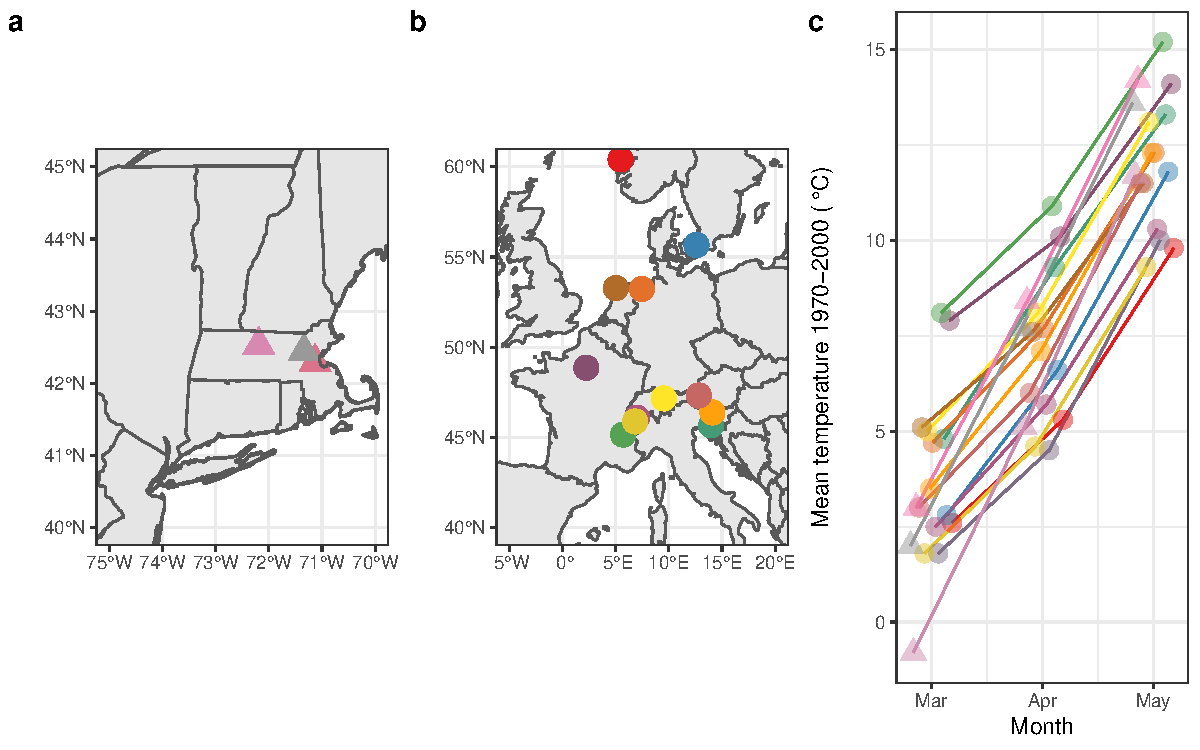
\includegraphics[width=1 \textwidth,trim=0cm 0cm 0cm 0cm, angle=0, scale=.9, origin=c,clip=false]{sampling_sites}}
		%x x x lower right 
		\caption{Map of collection sites of (A) invasive populations in New England and (B) native populations in Europe and (C) average Spring temperatures at each site}
		\label{fig:sites}
	\end{figure}

%	\begin{figure}
%		\centering
%		\fbox{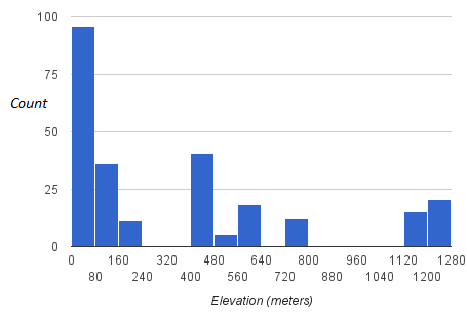
\includegraphics[width=1 \textwidth,trim=0cm 0cm 0cm 0cm, angle=0, scale=.7, origin=c,clip=false]{Elevation-chart}}
		%x x x lower right 
%		\caption{Count of European individuals collected at different altitudes. }
%		\label{fig:elev}
%	\end{figure}
	\subsection{Experimental Design}
	To test phenological responses to climate, seeds were exposed to eight treatments representing varying climates. Seeds were first subjected to one of two stratification treatments (varying length of stratification), and then planted in one of four temperature treatments. All treatments were carried out in growth chambers. For each treatment, ten representatives of each species (with seven invasive species this leads to 140 seeds per treatment) and an additional five representatives of each local population of \textit{Plantago lanceolata} (the most heavily sampled species, with 13 populations) leading to a total of 205 seeds per treatment. Germination, time to germination, and aboveground linear height were recorded. Local population representatives were drawn from the greatest variety of individuals (seed families), and the seed family representation was consistent across treatments. 
	
	\subsection{Stratification}
	Stratification is crucial for many species to break organic dormancy and germinate successfully \parencite{Baskin1998,Popay1970,Wulff1994} and winter length has been shown to drive ecological community shifts (Harte et al. 2015). Additionally, with changing climate, winter length is a key niche variable. Studies show stratification of our species vary from 16 days \parencite{Popay1970} to 120 days \parencite{Meekins1999}. This experiment thus used intermediate lengths of 30 and 60 days for our two stratification treatments. Seeds in the longer stratification treatment were stratified in late September 2015, while the other seeds in the shorter treatment continued to be stored in paper envelopes at room temperature until they were in turn stratified in late October 2015. Stratification conditions were kept constant across treatments:  4$^\circ$C, 70\% humidity, 380 ppm of $CO_2$ (the standard, see e.g., \textcite{Meekins1999,Popay1970}). Seeds were stratified on moistened Whatman 1 qualitative filter paper in Greiner bio-one 94x16 petri dishes (with vents, greiner light version, sterile) in the dark \parencite{Baskin1998,Popay1970} in a single Biochambers TPC-19 Reach-In Growth Chamber.  Water was added to petri dishes every 30 days.
	
	\subsection{Germination }
	On November 23, 2015, seeds from both stratification treatments were transferred from their petri dishes into individual pots with soil (see Experimental Design, above), which were placed into four different growth chambers (three Biochambers TPC-19 Reach-In Growth Chambers and one Biochambers LTCB-19 Reach-in Growth Chamber) and subjected to four different germination treatments. Temperature varied across treatments---all other measured variables were kept constant, and treatments were rotated through growth chambers to control for the unmeasured chamber effects. Seeds that germinated during stratifcation were discarded.
	
	\paragraph{Germination Temperature:} Popay and Roberts (1970) show that Capsella bursa-pastoris germinates best at 25-30$^\circ$C, and 20-30$^\circ$C seems to be the standard temperatures for optimal weed germination \parencite{Hartmann2010,Steinbauer1957,Wulff1994}. This experiment used a slightly-broadened spectrum to achieve a greater variance in germination success, using temperatures between 18 and 32$^\circ$C. 
	
	\paragraph{Thermoperiocity:} About 80\% of weeds studied in \textcite{Steinbauer1957} and about 75\% of cultivated seeds germinate better with thermoperiocity (i.e., daily fluctuations in temperature)\parencite{Toole1963,ISTA1954}. Thus thermoperiocity of 10$^\circ$C was used \parencite[see e.g.,][]{Steinbauer1957}, translating to treatment temperatures of: 18/8$^\circ$C, 22.67/12.67$^\circ$C, 27.33/17.33$^\circ$C, and 32/22$^\circ$C. All treatments were subjected to 8 hours at the high temperature and the remaining 16 hours at the low temperature \parencite{Baskin1998,Roberts1981,Popay1970,Probert2000}.
	
	
	\paragraph{Light type:} Germination rates typically increase when seeds are exposed to light \parencite[e.g.,][]{Baskin1998,Pons2000,Popay1970}. Different studies suggest that the ratio of far to far-red light (R:FR) matters either a lot or not at all for successful germination \parencite[e.g.,][]{Popay1970,Pons2000,Wulff1994}. But, generally, exposure to a high R:FR ratio, increases germination rates. Thus, our experiment used T5HO fluorescent lights \parencite{Toole1963}, which have a high R:FR ratio. 
	
	\paragraph{Period/luminance of light:} Some species have sufficient Pfr (the active form of phytochrome pigment, often necessary to induce germination) and so do not need any light to break dormancy, others just need a pulse of red light to break dormancy (the red light converts the inactive phytochrome into Pfr) \parencite{Casal998}.  Other species, including \textit{Plantago major}, take much longer to build up the requisite Pfr, and so have much higher germination success when exposed to longer periods of light (with nearly 100\% germination after 48 hours of exposure for \textit{P. major}) \parencite{Pons1991}. Finally, some species have a high irradiance response (HIR), germinating poorly when exposed to high luminance light or prolonged light \parencite{Roberts1987}. Beyond interspecific variation, there is also intraspecific variation in the relationship between dormancy and light \parencite{Probert1986}. Across all populations, germination rate seems to be log-normally related to photon dosage \parencite{Ellis1986}. Light may begin inhibiting germination for HIR species at about 0.1 mol/m\textsuperscript{2}/day--1 mol/m\textsuperscript{2}/day \parencite{Baskin1998,Ellis1986}, while other species peak above 10 mol/m\textsuperscript{2}/day \parencite{Ellis1986}. The differing levels of light necessary to break dormancy means that any chosen light regime will be better for some species and worse for others. 
	
	The goal of these experiments is to create germination rates that are sufficient to observe variation in responses to treatments. Thus, we chose an intermediate light exposure at which all of the species should germinate at substantial levels, but which may not be ideal for any species. In selecting how much light to use, this experiment erred on the side of too much light rather than not enough, since at least one of our species is known to need large amounts of light (\textit{Plantago major}---\textcite{Pons1991}), and none are known to exhibit HIR (although a \textit{D. glomerata} subspecies in southern Europe does exhibit HIR \parencite{Probert1986}, but this subspecies is not thought to have been collected for this study). Thus this experiment used a length of eight hours at a luminance of 75 micromol/m\textsuperscript{2}/second to yield a daily photon dosage of 2.16 mol/m\textsuperscript{2}. \textcite{Baskin1998} recommend that the light period coincide with the high-temperature period. Thus, this experiment exposed the seeds to eight hours of fluorescent light during the high-temperature thermoperiod. 
	
	\paragraph{Substrate and planting depth:} \textcite{Popay1970} show that \textit{C. bursa-pastoris} seeds germinated about equally on filter paper as on top of soil, but showed much decreased germination when inserted into soil. The effects of planting substrate and depth have not been studied in most of the study species. However, a study on a species related to \textit{D. glomerata} suggests that \textit{D. glomerata} may germinate better in soil \parencite{Andrews1974}. Additionally, a difference in depth of just a couple millimeters can result in extreme differences in light availability \parencite{Tester1987}. Thus each seed was placed on top of Fafard Growing Mix (a mixture of fine peat moss, fine perlite, and vermiculite) soil, with each seed in its own individual tray cell.
	
	\paragraph{Water:} Every two days, seeds were watered until all of the soil had become wet \parencite{Steinbauer1957}; but not so much that a film of water covered the seeds \parencite{AOSA1960}.
	
	\paragraph{Germination monitoring:} Seeds were checked during the light period for germination every two days. Germination success was defined as the growth of shoot or radical through the seed coat \parencite{Baskin1998,Popay1970}. Germination date for each seed was recorded. Data collection sheets only contained the tray location of the seeds, (not population or individual), so collection of germination data was blind to population.  Germination trials typically last two weeks, with most seeds germinating within 10 days \parencite{Baskin1998}. However, after 10 days, new germinations were still being observed so the observation time was extended \parencite{Wulff1994}.
	
	\subsection{Growth}
 	Most of the study species are perennials or biennials. As such, they do not flower in the first year. Instead of floral state, each plant's height was measured. Aboveground linear height of each seedling was measured five times: on December 7, 2015, December 15, 2015, December 21, 2015, January 4, 2016, and January 29, 2016. On January 1, 2016, the plants were moved from the growth chambers to a greenhouse subject to the following conditions: natural photoperiod (approximately 10 hours of light/day), 20 to 25$^\circ$C, and 65\% humidity.  
 	

	\subsection{Statistical analysis}
	Height was linearly associated with day, so growth rate (in cm/day) was defined as $\beta$ in the linear model: $height = \alpha + \beta*day $ (see Figure SXX). This growth rate was calculated for each seed that germinated. Treatment effects on growth rate, germination rate, and germination timing were modeled with Bayesian multilevel models \parencite{Gelman2004}. For all models, stratification length, continental origin, and temperature were treated as binary fixed effects. Europe, 18/8$^\circ$C, and 30 days were reference levels for origin, temperature, and stratification length, respectively; temperature was recoded as three dummy binary factors. The full suite of 2- and 3-way interactions were included for all fixed effects. Seed family was treated as a random effect, nested within sampling population, nested within species (with random slopes and intercepts). Growth rate was modeled with a normal error distribution: 

\begin{align}
y_i =&  N(\mu_i,\sigma)\\
  \mu_i =&  \alpha_{sp[pop[sfamily[i]]]} + \beta 1_{sp[pop[sfamily[i]]]}\times origin +  \beta 2_{sp[pop[sfamily[i]]]} \times strat\\
          & +\beta 3_{sp[pop[sfamily[i]]]}\times temp1 +  \beta 4_{sp[pop[sfamily[i]]]}\times temp2 + \beta 5_{sp[pop[sfamily[i]]]}\times temp3 \notag \\
          & 
 		 + \beta 6_{sp[pop[sfamily[i]]]}\times origin\times strat  + \beta 7_{sp[pop[sfamily[i]]]}\times origin \times temp1 \notag\\ &
 		 + \beta 8_{sp[pop[sfamily[i]]]}\times origin \times temp2 + \beta 9_{sp[pop[sfamily[i]]]}\times origin \times temp3 \notag \\ &
 		 +\beta 10_{sp[pop[sfamily[i]]]}\times strat\times temp1 +\beta 11_{sp[pop[sfamily[i]]]}\times strat \times temp2 \notag \\ &
 		 + \beta 12_{sp[pop[sfamily[i]]]}\times strat \times temp3_ + \beta 13_{sp[pop[sfamily[i]]]}\times origin \times strat \times temp1 \notag\\ &
 		 +\beta 14_{sp[pop[sfamily[i]]]}\times origin \times strat \times temp2 + \beta 15_{sp[pop[sfamily[i]]]}\times origin \times strat \times temp3 )\notag
 \end{align}
 \begin{align}
 		 \intertext{Where the $\alpha$ and each $\beta$ coefficient were specified with nested random effects. For each $\gamma$ in $[\alpha,\beta 1:\beta 15]$:}
 		 \gamma_{sp[pop[sfamily[i]]]} =& N(\mu_{\gamma_{sp[pop[j]]}}, \sigma_{\gamma_{sp[pop[j]]}}) \\
 		 \gamma_{sp[pop[j]]} = & N(\mu_{\gamma_{sp[k]}}, \sigma_{\gamma_{sp[k]}}) \\
 		 \gamma_{sp[k]} = & N(\mu_{\gamma}, \sigma_{\gamma})
\end{align}


	 Where $sp = $ species, indexed with $k$, $pop =$ sampling population, indexed with $j$, $sfamily =$ seed family, indexed with $i$, and $strat$ = stratification. Germination rate was modeled similarly to growth rate, but using a binomial error distribution and logit link function, while germination timing was modeled with a Poisson error distribution and log link function. 
	 	
	All models were estimated using four chains, each with 2000 iterations (including 1000 devoted to warm-up), and wide priors. All models were built with Stan \parencite{Carpenter2017} using rstanarm version 2.17.4 \parencite{Goodrich2018} in R \parencite{Team2015}. Chain convergence was confirmed using the Gelman-Rubin statistic/$\hat{R}$ close to one \parencite{Gelman1992}. Models implementations were validated using simulated data; model fits were assessed using posterior predictive checks \parencite{Gelman2004}.  
	
	\paragraph{Average predictive comparisons} The interactions and random effects make this model complex, and frustrate clear interpretation of parameter estimates. Average predictive comparisons can increase interpretability of variables in complex models \parencite{Gelman2007}. Across interaction terms and mixed effects, this method is capable of providing a single point estimate and associated uncertainty of the impact of a given parameter. Additionally, unlike model output from Poisson and Binomial models which are given in transformed units, average predictive comparisons yield estimates that are in the units of the dependent variable \parencite{Gelman2007}. Average predictive comparisons translate the variability in parameter draws directly into uncertainty in estimates \parencite{Gelman2007}. This makes average predictive comparisons well-suited for complex Bayesian models. However, despite being theoretically introduced more than a decade ago, average predictive comparisons remain complicated to implement. However, our stratification and temperature variables are balanced and independent  (i.e., every combination of input values is equally likely to co-occur), so we can ignore average predictive comparison's weighting requirement, thus simplifying the computation. We therefore calculate average predictive comparisons for stratification and each temperature factor.
	
	\paragraph{Data, code} 
	Data and R code is available on github at ??
	\section{Results}
	\paragraph{Germination rate} Germination rate was high: 0.76\% of seeds germinated. Overall, germination rate was insensitive to temperature, stratification, or origin---95\% credible intervals (CrI) for all effects were clustered around zero (Figure \ref{fig:coef}). Regardless of the climatic conditions that we presented the seeds with, they germinated at fairly constant, high rates. Seeds from the invasive and native ranges germinated at similar rates and responded similarly to treatments. Seeds from different local populations also germinated at similar rates (see Figure SXX).
 %(95\% CrI: round(invlogit(mod_rate$stan_summary[2,4]),2)--round(invlogit(mod_rate$stan_summary[2,10]),2))
	\paragraph{Germination timing} The mean time to germination was 12.33 days.  Overall, all species germinated slower at the lowest temperature, but germinated at similar, faster speeds at the three higher temperatures, showing that temperature response is non-linear  (see Figure \ref{fig:coef}). Overall,stratification and seed origin had no noticeable effect; however, PLALAN did show faster germination in response to med-low temperature $\times$ stratification interaction (see Figure SXX).  Additionally, there was a significant positive interaction effect of origin, stratification and the higher temperature (95\% CrI: 1.05--2.9 days). Populations showed fairly homogeneous responses, though temperature $\times$ stratification interactions did show some inter-population variability (see Figure SXX). 
	
	\paragraph{Growth rate} The mean growth rate was 1.2 mm/day. Overall, growth rate was the most sensitive to treatments, though it still did not exhibit main-effects responses to stratification or origin (see Figure \ref{fig:coef}). Growth rate decreased at warmer temperatures for all species, but especially DACGLO. This response to temperature was more linear than that observed in germination timing. These contrasting responses of germination timing and germination growth is made even more clear by the results of the average predictive comparisons, which, in units of the predictors, shows that each of the higher temperatures had indistinguishable effects on germination timing, but sequentially bigger effects on growth rate (see Table \ref{tab:apc}).  However, this substantial growth rate decrease at the highest temperatures was moderated in seeds stratified for 60 days and originating in North America (the invasive range): these plants grew 7.43mm faster per day (95\% CrI: 2.18--12.73).
	%Across germiantion rate, germination timing, and growth rate, seeds from the invasive and native ranges responded similarly to temperature and stratification treatments. 

% latex table generated in R 3.5.1 by xtable 1.8-3 package
% Mon Jan 20 11:15:45 2020
\begin{longtable}{rlll}
\caption{Average predictive comparisons provide an additional interpretation of the results. They show, on average, how much change in the dependent variable results from a one unit change in the predictor variable.}.
\label{tab:apc}\\
	\hline
	variable & germination rate (fraction) & germination date (days) & growth rate (cm/day) \\ 
	\hline
	stratification & 0.436 $\pm$ 0.023 & 9.629 $\pm$ 0.52 & 0.042 $\pm$ 0.002 \\ 
	temperature 1 & 0.388 $\pm$ 0.033 & 10.244 $\pm$ 0.343 & 0.029 $\pm$ 0.003 \\ 
	temperature 2 & 0.394 $\pm$ 0.032 & 10.196 $\pm$ 0.347 & 0.079 $\pm$ 0.003 \\ 
	temperature 3 & 0.38 $\pm$ 0.032 & 10.304 $\pm$ 0.337 & 0.091 $\pm$ 0.003 \\ 
	\hline\\
	\hline
\end{longtable}

\begin{figure}
	\fbox{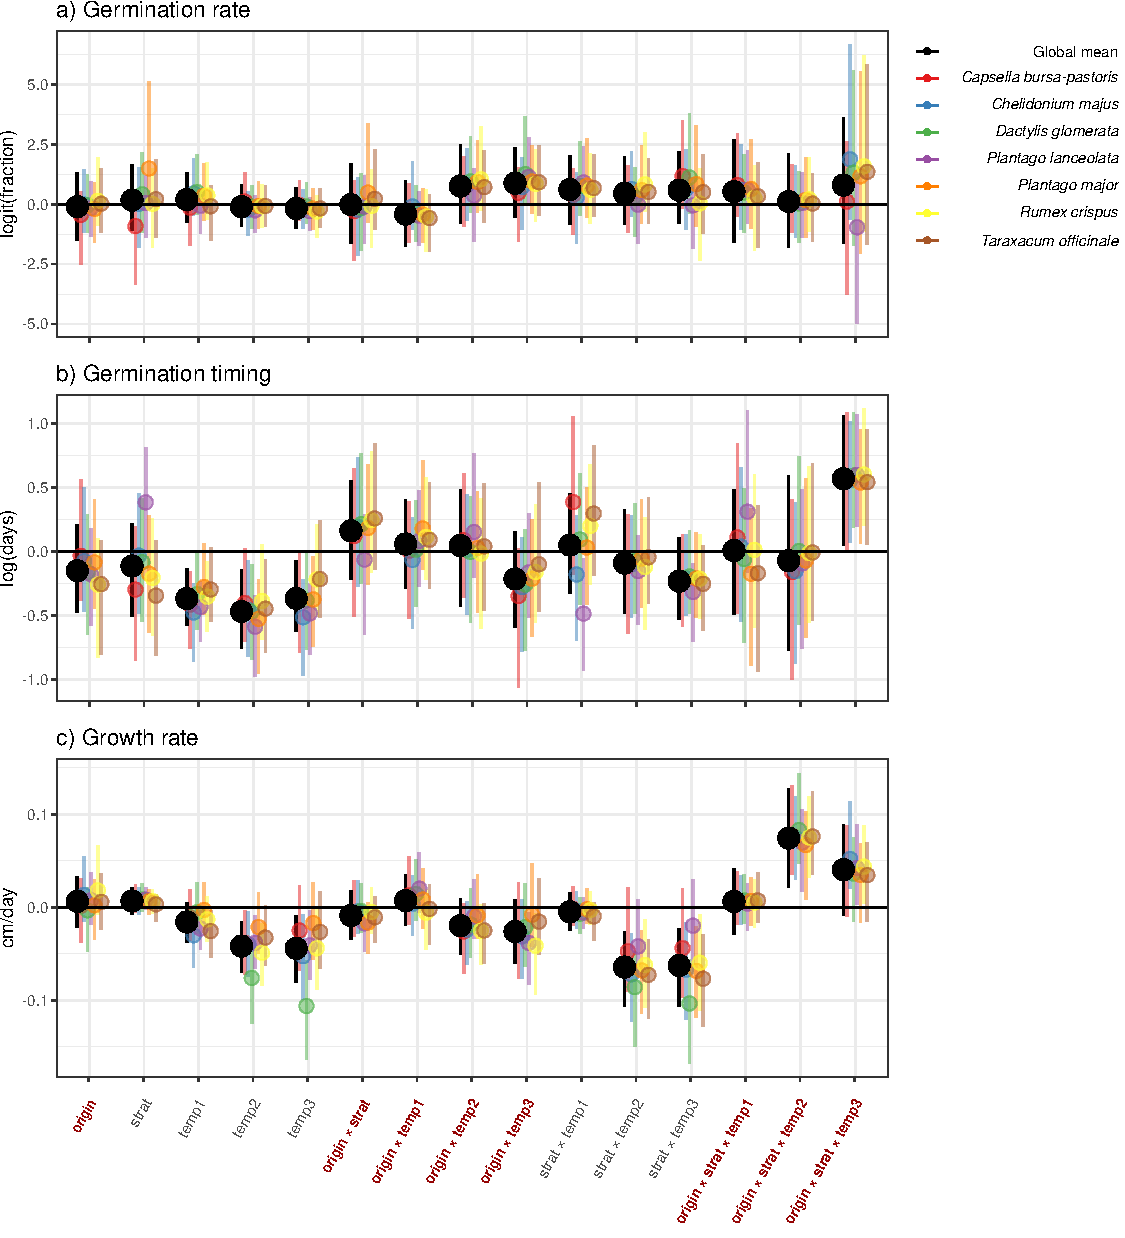
\includegraphics[scale=.5,angle=-90]{germ_figs_onepage.pdf}}
	\caption{Multilevel model coefficients with 95\% credible intervals, showing global average effects and species random effects. Intercept coefficients not shown.  a) model of germination rate, b) model of germination timing and c) model of growth rate}
	\label{fig:coef}
\end{figure}

	\section{Discussion} 
	
	This study leveraged the power of a multi-species growth chamber experiments of native and introduced populations to investigate the importance of rapid evolution for invasive success. Across seven highly invasive plant species, we found only isolated support for the prevalence of post-introduction rapid evolution. Instead, our results support the theory that species do not need to evolve to invade: weediness, wide environmental tolerance, plasticity, or generalist traits in the source populations likely provide sufficient capacity to exploit novel environments \parencite{Baker1965}. Rapid evolution may provide a helping hand, but contrary to the many claims about the essentiality of rapid evolution in invasive species, it but may not be the dominant technique for invasion success.  
	
	These findings are  especially pronounced in germination rate, where all species germinated well and with scant sensitivity to climatic conditions, suggesting that the source populations of invading species provided invaders with the capacity to germinate in any environment, without the need to evolve. Some have suggested that while initially species may not need to evolve, they may once achieving a foot-hold \parencite{Lamarque2015}. However, many of our study species (e.g., DACGLO) have occupied their invasive range for centuries, yet still show little sign of an evolving germination response. 
	
	Overall, germination timing and growth rate also showed that species have not evolved upon becoming invasive. However, there was some evidence that particular responses have evolved: North American (invasive) populations appear to have evolved to germinate later and grow faster under high-temperature/long stratification combinations. Taking the climate of our North American populations into account (Figure \ref{fig:sites}), this growth rate evolution may be adaptive. Our North American populations experience climates with longer winter stratification  (lower mean March temperatures) and hotter growing temperatures (higher mean May temperature). Thus, the capacity to grow faster at high temperatures after being exposed to our long stratification treatment may provide fitness advantages. Although it is  possible that these differences could be residual founder effects \parencite{Shirk2014}, a result of genetic drift \parencite{Eckert1996}, or that germination rate is not a fitness trait,  the convergence with experienced climate suggests that this observed change in growth rate is a sign of isolated adaptive evolution. 
	
	These changes may also suggest that these invasive species may be able to adapt to changing climates. Because cold-stratification is a simulation of temperate winter, the evidence that species can adapt their growth rate in accordance with winter length and spring temperature suggests that they may have the capacity to adapt to changing winter lengths and spring temperatures that anthropogenic climate change is bringing \parencite{IPCC2015}. These results also echo the  importance of varying both winter length and spring temperature in order to obsrve responses to climatic \parencite[e.g.,][]{Bernareggi2016}. Future studies can build upon the seven species presented here to see the extent to which these generalizations persist. Moreover, future studies should also include biotic factors, since these can be very important for preventing, or enabling, invasions \parencite{Germain2018}. 
	
As a rule, rapid evolution is not essential for invasion success. But rapid evolution may still play a role, especially in more extreme or different environments:  \textcite{Linde2001} found that CAPBUR evolved to colonize high-altitude and desert environments in California. However, we found little sign of evolution in our comparisons between temperate populations of this species. Future work could explore the types of circumstances when rapid evolution may be more or less important. Perhaps, as suggested by Baker (1965), the generalist traits contained in temperate source populations are suitable as long ss the introduced environment is not too different. Our findings provide support for  the speculation by van Kleunen and colleagues (2010) that future invasions can be predicted by species' characteristics. This finding suggests that managers can perhaps best guard against future invasions by targeting weedy species and preventing them from dispersing beyond their native ranges. 
	
	
	\section{Acknowledgments}
	 This field work was supported by the Harvard College Research Fund and the Harvard University Center for the Environment Undergraduate Summer Research Fund. Thanks to Beth Forrestel for mentorship to HNE. Thanks to J. Williams and H. Branch for fruitful discussions. Thanks also to D. Flynn, S. Gee, J. Samaha, and T. Savas for help transplanting, collecting, and measuring. Thanks to F. Rosin, K. Woodruff, and J. Gard for help with collection and growing logistics. Thanks to S. Fritz for help with data input. Thank you to M. Rucinski, C. Husic, N. Gilbert, A. Delgado, and A. Acosta for comments on earlier drafts of this paper. Thanks to J. Eyster, S. Stalhandske, and G. Barbone for assistance with and camaraderie during field sampling. 

	

\section{Literature Cited}
\printbibliography
\end{document}
